\section{Entwurf}

\label{sec_impl_architecture}

\todo{Einführender Absatz}

\subsection{Eingriff in den Datenfluss des SIEM-Systems}

\todo{Hier allgemein - OSSIM erst in 5.1.}

Für den Eingriff zur Pseudonymisierung der Logdaten bieten sich verschiedene Stellen im Datenfluss eines SIEM-Systems an. In diesem Abschnitt sollen die verschiedenen Möglichkeiten dargestellt und gegeneinander abgewogen werden. Eine Übersicht über die verschiedenen Stellen bietet Abbildung \ref{fig:siem_data_access_point}. Im Folgenden sollen diese Möglichkeiten bezogen auf die in Abschnitt \ref{subsec_impl_requirements_ossimintegration} dargestellten Eigenschaften\todo{EZ: Kannst du nochmal kurz sagen, um was fuer Eigenschaften es da ging? Ich weiss es jetzt schon nicht mehr.} bewertet werden.

\todo{EZ: Es ist nicht gleich klar, dass sich diese Aufzaehlung auf die Nummern in der Abbildung beziehen.}

\begin{enumerate}

\item \textbf{In der Quelle der Logdaten}\\
  Bei diesem Ansatz werden die Daten bereits pseudonymisiert, bevor sie die Datenquelle verlassen. Dieser Ansatz würde dafür sorgen, dass die Daten bereits pseudonymisiert auf der Übertragungsstrecke und im SIEM-System vorliegen. Es wäre kein mehrfaches Parsen der Daten notwendig und der Ansatz wäre unabhängig vom verwendeten SIEM-System. Auf der anderen Seite würde dieser Ansatz die universelle Veränderung jeder Datenquelle notwendig machen. 
  Auch wenn dieser Ansatz aus datenschutztechnischer Sicht die beste Möglichkeit darstellen würde, so ist er doch nicht umsetzbar, da hierzu jede mögliche Quelle von Logdaten universell verändert werden müsste.
  \todo{EZ: Hier machst du es dir ein bisschen zu einfach. In deinem Log-Proxy musst du ja auch alle moeglichen Logs, die dort ankommen, universell veraendern. Was spricht also dagegen, dass man diesen Proxy einfach lokal auf jeder Logquelle laufen laesst? Dann braeuchte nicht mal mehr die Searchable Encryption. Denn der lokale Proxy sieht ja immer wieder das gleiche identifizierende Merkmal und kann sich dazu einfach eine Tabelle aufbauen mit den zugehoerigen Pseudonymen. Das kann im Klartext passieren, da die Merkmale auf der Logquelle ja sowieso im Klartext sichtbar sind.}

\item \textbf{Proxy-basierter Ansatz}\\
  Dieser Ansatz pseudonymisiert die Daten vor dem ersten Kontakt mit dem SIEM-System, indem Datenquellen ihre Logdaten an einen Proxy senden, der die Daten pseudonymisiert und erst anschließend an das SIEM-System weiterreicht. Hierdurch wird erreicht, dass die Daten zu keiner Zeit nicht-pseudonymisiert in dem SIEM-System vorliegen. Außerdem ist er unabhängig von Datenquellen und SIEM-System und erfordert keinen direkten Eingriff in diese (abgesehen von geringen Konfigurationsanpassungen). Ein Nachteil dieser Lösung ist, dass sie das Parsen und Neuzusammensetzen der Logdaten im Proxy zusätzlich zu deren anschließender Behandlung im SIEM-System erfordert.

\item \textbf{Patchen des SIEM-Systems}\\
  Die letzte Möglichkeit ist das Verändern des SIEM-Systems selbst. Hierzu wird in die Logdaten parsende Komponente eingegriffen, um vor, während oder nach diesem Vorgang die Logdaten zu pseudonymisieren. Dieser Ansatz erfordert kein mehrfaches Bearbeiten von Logdaten wie in dem Proxy-basierten Ansatz. Auf der anderen Seite ist er abhängig vom eingesetzten SIEM-System und erfordert seine Veränderung. Zusätzlich liegen die Daten erst einmal in nicht veränderter Form im SIEM-System vor, was die in Abschnitt \ref{subsec_impl_requirements_ossimintegration} erwähnten Nachteile mit sich bringt.

\end{enumerate}

\begin{figure}[]
    \centering
        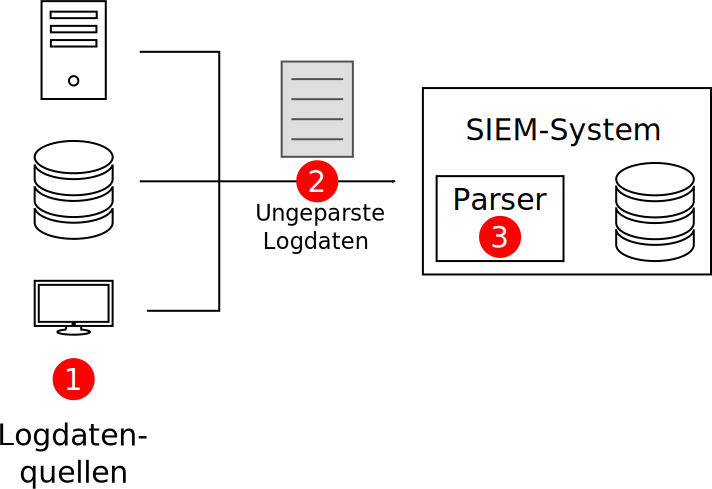
\includegraphics[width=0.5\textwidth]{dia/siem_data_access_point.pdf}
    \caption{Mögliche Eingriffspunkte in den Datenfluss eines SIEM-Systems.}
    \label{fig:siem_data_access_point}
\end{figure}

Insbesondere der aus datenschutztechnischer Sicht relevante Vorteil, dass die Daten bereits pseudonymisiert in dem SIEM-System eintreffen, ließ die Entscheidung auf die \textbf{zweite Möglichkeit} fallen. \todo{Digitalgipfel:   Die	 Pseudonymisierung	 ist	 im	 Verarbeitungsprozess	so	früh	wie möglich	durchzuführen.	 }
Dass die Lösung außerdem noch keine Anpassungen an dem SIEM-System selbst erfordert, wiegt den Nachteil des zusätzlichen Parsens und wieder Zusammensetzens der Lognachricht bei Weitem auf.\todo{Auch auf Angreifermodell beziehen}



\subsection{Architektur}

%- Beschreibung Architektur
%
%- Wie deckt dieser Ansatz die Anforderungen ab?
%  - Einbindung OSSIM
%  - Pseudonymisierung
%  - Schwellwert
%  - Benutzerinteraktion
%  - Erweiterbarkeit Datenquellen
%  - Erweiterbarkeit Datenschutztechniken

\todo{Hier erweitern: 
Warum verteilte Lsg (ProxyPlugin - Service):
  - Erweiterbarkeit (Mehrere Proxy-Server mit verschiedenen Protokollen, evtl. auch direkt Client-seitig, ...) => Absicherung einer Komponente, die jedoch auch nicht alles erfährt
  - Trennung Verarbeitung und Speicherung (Kompr. DB -> Pseudonyme bleiben verdeckt, Kompr. Proxy -> bisherige Daten und Daten evtl. anderer Proxys bleiben abgesichert)
}

Ausgehend von diesen Überlegungen wurde ein verteiltes System entworfen, dass die Anforderungen aus Abschnitt \ref{sec_impl_requirements} erfüllt und an der beschriebenen Stelle in den Datenfluss eingreift. 
Einen Überblick bietet Abbildung \ref{fig:high__level_architecture}. Das System besteht aus verschiedenen Komponenten, die im Folgenden näher beschrieben werden.

\begin{figure}[]
    \centering
        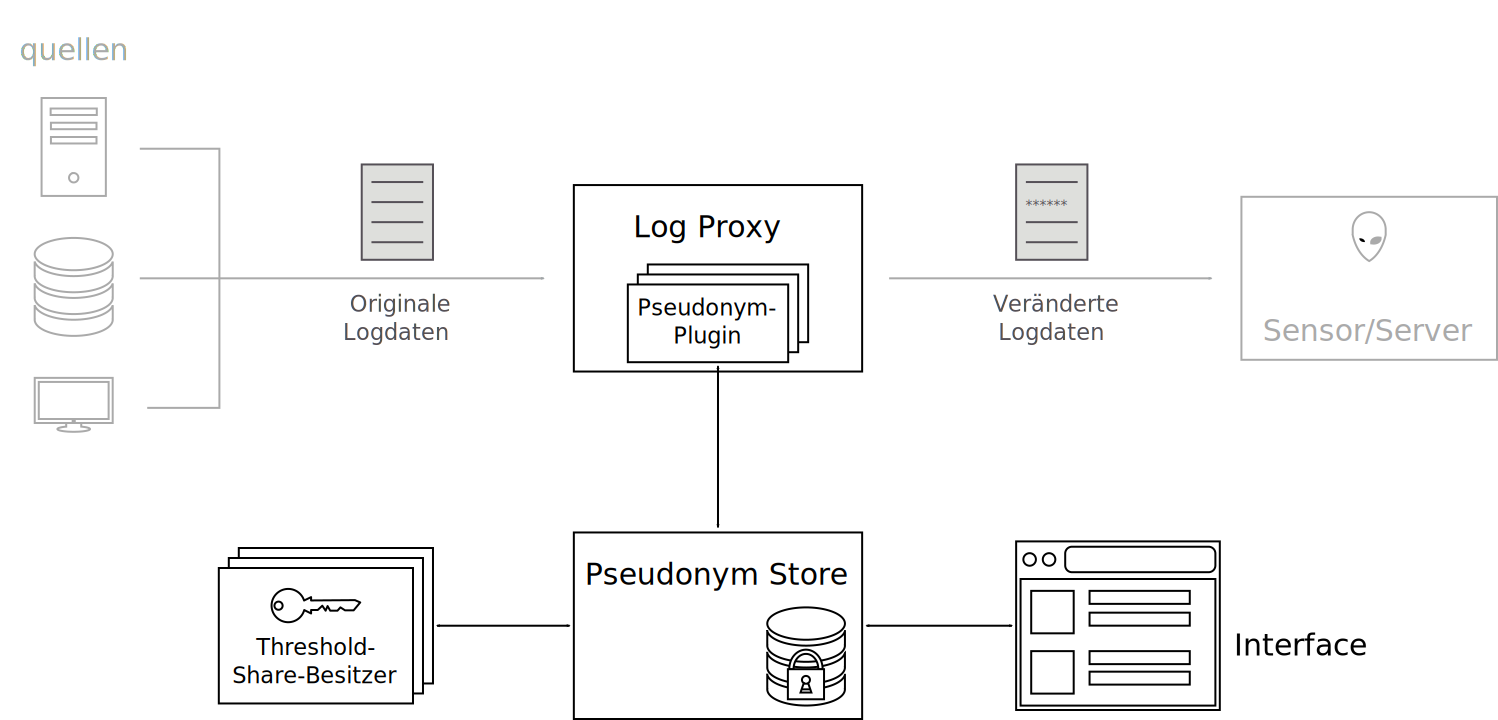
\includegraphics[width=0.9\textwidth]{dia/high_level_architecture.pdf}
    \caption{Ein Überblick über die entworfene Architektur.}
    \label{fig:high__level_architecture}
\end{figure}

Ein \textbf{Log-Proxy}, der die Daten über das Syslog-Protokoll entgegennimmt, verändert und anschließend an OSSIM weiterleitet. Das Verändern der Daten kann mit verschiedenen Plugins geschehen, so dass neben der umzusetzenden Pseudonymisierung auch weitere Datenschutztechniken eingesetzt werden können, was die geforderte Erweiterbarkeit aus Abschnitt \ref{subsec_impl_requirements_plugins} ermöglicht. Der Proxy leistet die Behandlung von Logdaten aus verschiedenen Quellen (siehe Abschnitt \ref{subsec_impl_requirements_differentsources}), was wie bereits im vorhergehenden Abschnitt beschrieben durch Parsen und Wiederzusammensetzen der Daten geschehen muss. Die Konfiguration des quellenabhängigen Vorgehens bei der Logdatenverarbeitung erfolgt ebenfalls hier.

Ein in dem Proxy enhaltenes Plugin wird für die Pseudonymisierung von Daten zuständig und kommuniziert dazu mit einer externen Komponente -- dem Pseudonym-Service. Die Kommunikation mit dem Proxy erfolgt über einen Webservice-basierten Ansatz. Das Plugin kann für eingehende Daten ein Pseudonym anfordern und dieses anschließend in den Logdaten verwenden.

Der \textbf{Pseudonym-Service} erfüllt zwei Aufgaben: das Speichern und Verwalten der Pseudonyme sowie die Integrierung des kryptographischen Schwellwertschemas. Initial muss die Schlüsselgenerierung des Schwellwertschemas (bei zentraler Schlüsselgenerierung) oder die Koordinierung der teilnehmenden Benutzer (bei dezentraler Schlüsselgenerierung) durch den Service geleistet werden. 
Es können während des Betriebs neue Pseudonyme angelegt und zusammen mit ihrem durch das Schwellwertschema verschlüsselten Datum abgelegt werden. Sie werden durch geeignete Maßnahmen durchsuchbar gehalten, um für ein Datum überprüfen zu können, ob bereits ein Pseudonym vergeben wurde. 
Über ein Webinterface kann ein berechtiger Benutzer die Aufdeckung eines bestimmten Pseudonyms fordern und den Status seiner Forderung bzw. im Erfolgsfall das aufgedeckte Datum betrachten. Dieses Datum wird durch das Kombinieren der partiellen Entschlüsselungen erhalten, die von den entsprechenden \textit{Share}-Besitzern berechnet werden.

Benutzer, die zuständig für die Bewertung von Anfragen zur Aufdeckung eines Pseudonyms sind, erhalten die Möglichkeit zur Interaktion mit dem System über eine \textbf{Client-Anwendung}, für die der Pseudonym-Service ebenfalls als Webservice agiert. Diese Anwendungen leisten im Falle der dezentralen Schlüsselgenerierung die initiale Generierung, verwalten den \textit{Share} des Benutzers und können nach der Bestätigung des Benutzers zu der Aufdeckung eines Pseudonyms partiell beitragen. 
